% leftover from chapter 1: consider inserting here or delete
%\footnote{Les deux affirmations appelées \wfd{Principe zéro de la thermodynamique}{principe zéro} et \wfd{Troisième principe de la thermodynamique}{troisième principe} sont beaucoup moins intéressantes et n’ont aucune conséquence pratique pour l’ingénieur/e}

\section{Le second principe}

	\subsection{Énoncé}

		Le \vocab{second principe de la thermodynamique} s’exprime ainsi :

		\begin{principe}
		La chaleur ne se déplace spontanément\hspace{\stretch{1}}\hspace{1ex} \\		
		\hspace{1ex} \ \hspace{\stretch{1}} que vers une température plus basse.
		\end{principe}

		On peut préciser cette affirmation de la façon suivante :

		\begin{trucimportant}
		Le transfert de chaleur vers une température plus haute\linebreak
		ne peut se faire sans apport d’énergie.
		\end{trucimportant}

		Nous allons voir que ce simple constat a des conséquences multiples et profondes pour l’ingénieur/e. En particulier, il détermine l’efficacité maximale de tous les moteurs et réfrigérateurs !



	\subsection{De l’évidence du second principe}

		Il est facile de s’offusquer tant l’énoncé ci-dessus paraît évident. Deux remarques s’imposent ici.

		\begin{itemize}
			\item Le second principe peut être énoncé de multiples façons. On parle plus souvent d’«~accroissement de l’entropie~» que du comportement spontané de la chaleur ; pourtant ces différents énoncés, que nous aborderons progressivement, sont tous équivalents.
			\item L’apparente évidence manifeste du postulat --\ on se doute que nul n’a jamais vu de tasse de thé chaud se réchauffer spontanément, ni de boisson fraîche se refroidir seule à température ambiante\ -- s’effrite dès que l’on étudie les phénomènes à l’échelle microscopique. 

		En effet, si la température n’est que le niveau d’agitation des particules, alors rien n’empêche \textit{a priori} celle-ci d’augmenter localement même si la température ambiante est plus faible\footnote{L’étudiant/e curieux/se pourra explorer cette idée en étudiant l’expérience fascinante du Démon de Maxwell, qui ouvre les portes à de nombreux nouveaux concepts.}. Il a fallu un demi-siècle de travail ardu aux thermodynamiciens pour répondre à cela de façon satisfaisante\footnote{C’est l’application des probabilités à la thermodynamique (même si l’on parle bien de thermodynamique statistique) qui permettra de la réconcilier avec la vision Newtonienne du monde, au cours du \textsc{xx}\ieme siècle.}. Il ne s’agit pas d’un problème trivial.
		\end{itemize}

		Dans notre étude et depuis notre point de vue d’ingénieur/e, nous accepterons le postulat ci-dessus comme une évidence, sans chercher ni à le justifier, ni à l’expliquer.

		 
	\subsection{Tous les moteurs rejettent de la chaleur}
	\label{ch_démo_second_principe}

		Imaginons vouloir créer du travail en prenant de la chaleur à un objet «~chaud~», c’est-à-dire à haute température : par exemple, \SI{100}{\degreeCelsius}, comme montré en \cref{fig_démo_second_principe_1}. On y accole un fluide dans un cylindre, que l’on laisse pousser sur un piston au fur et à mesure qu’il reçoit de la chaleur.

		\begin{figure}
			\begin{center}
				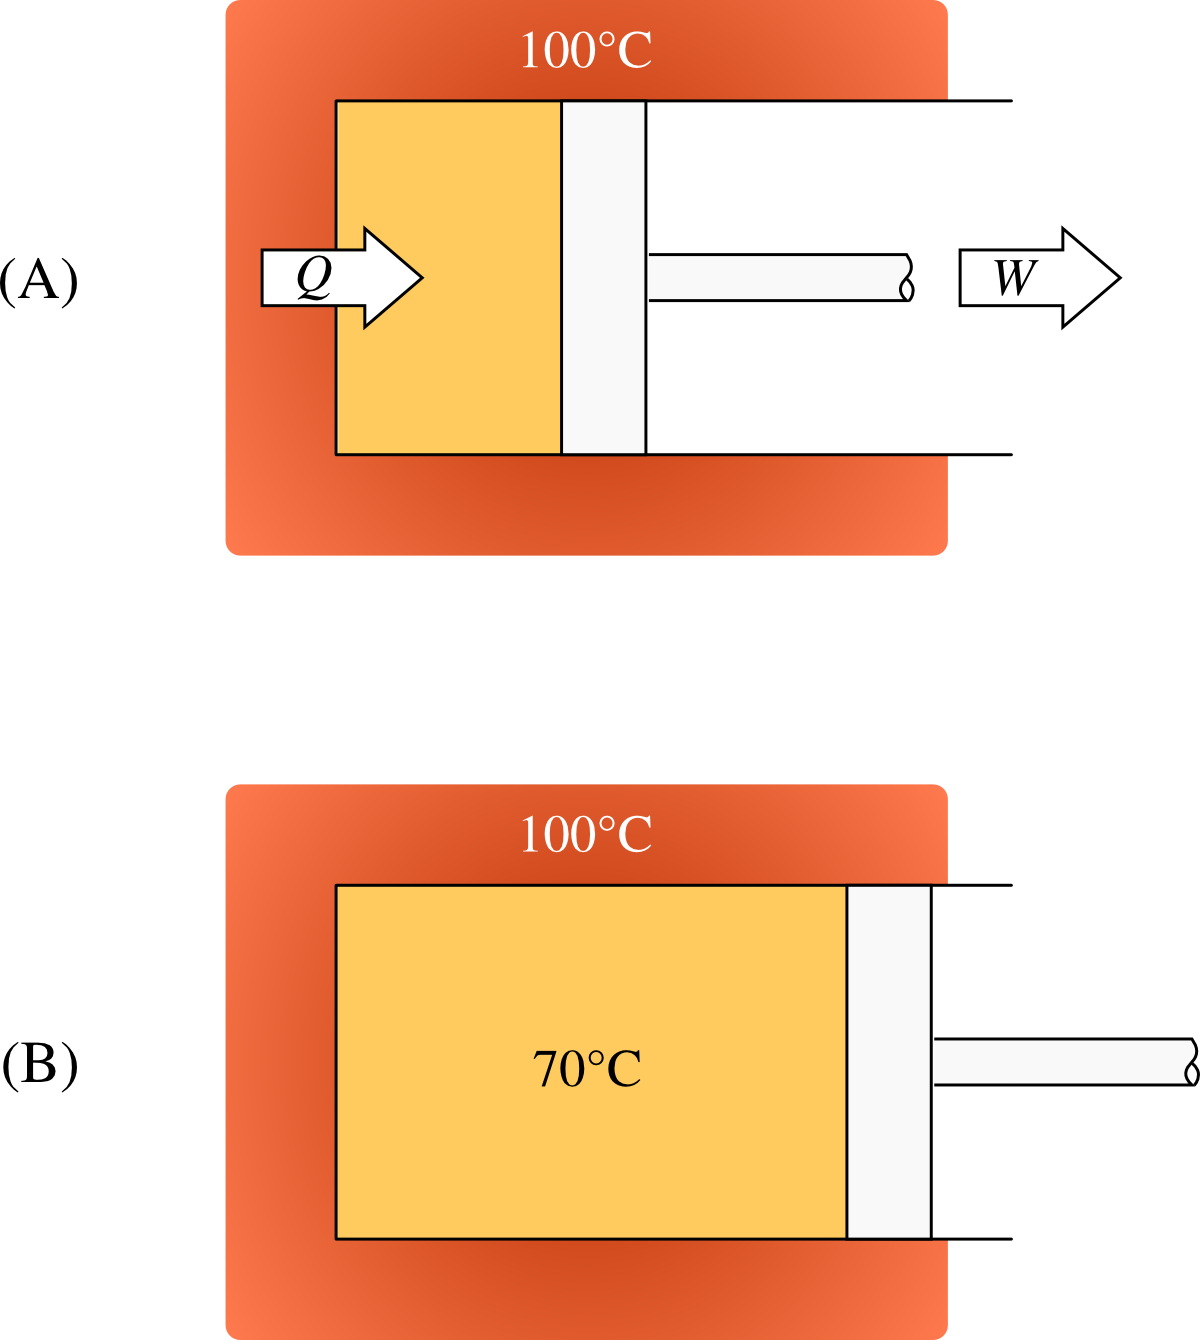
\includegraphics[width=8cm]{images/demo_second_principe_1.png}
			\end{center}
			\caption{Production d’un travail avec de la chaleur issue d’un corps à~\SI{100}{\degreeCelsius}.}
			\label{fig_démo_second_principe_1}
		\end{figure}

		Une fois qu’une quantité de travail a été fournie (en B sur la \cref{fig_démo_second_principe_1}), le fluide a augmenté de volume. Si nous souhaitons continuer à transformer de la chaleur en travail, et que nous ne souhaitons pas que le moteur «~gonfle~» indéfiniment, il nous faut refroidir ce gaz pour le ramener à son volume initial.

		Malheureusement, \emph{la seule façon} d’extraire de la chaleur du gaz est de le mettre en contact avec un corps plus «~froid~», comme montré en \cref{fig_démo_second_principe_2}. Il est notamment impossible de restituer la chaleur accumulée dans le gaz au corps «~chaud~» --\ il faudrait pour cela que la température du gaz soit plus grande que lui\footnote{Notons qu’en poussant le raisonnement à ses limites, le moteur pourrait recevoir et fournir la chaleur à température constante. Mais alors, le travail à fournir pour ramener le fluide à son état initial serait exactement le même que celui développé pendant la détente : le cycle ne transformerait effectivement pas de chaleur en travail, et ne présenterait alors pas d’intérêt pratique.}\nolinebreak.

		\begin{figure}
			\begin{center}
				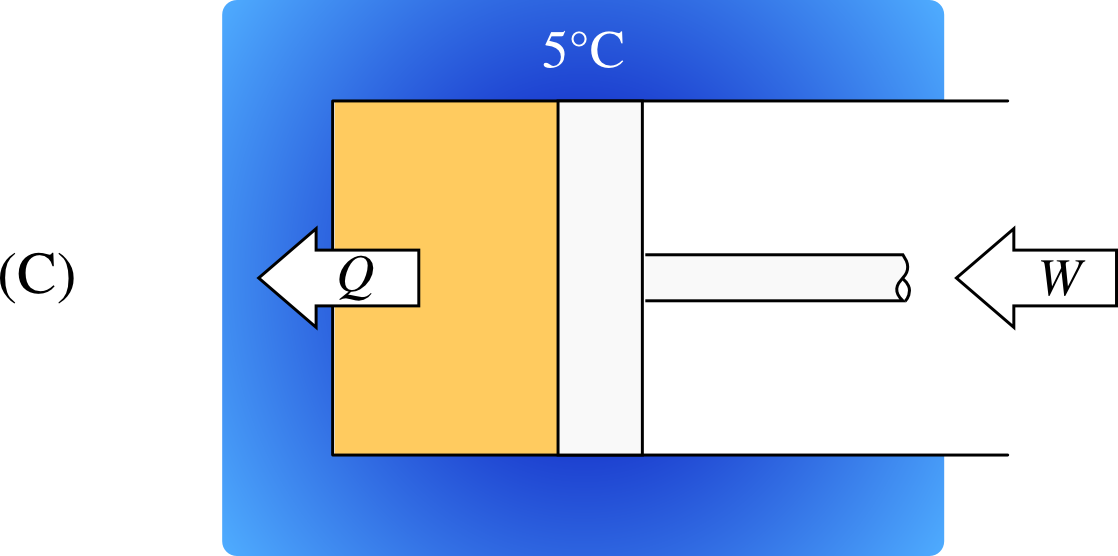
\includegraphics[width=7.2cm]{images/demo_second_principe_2.png}
			\end{center}
			\caption{Le refroidissement inévitable du moteur.
		La seule manière de ramener le fluide à son état initial (A) dans l’expérience en \cref{fig_démo_second_principe_1} est de lui prélever de la chaleur, ce qui ne peut se faire qu’avec un «~puits~» à chaleur de température plus basse. Les transferts de chaleur et de travail sont ici plus faibles qu’à l’aller, mais tous deux non nuls.}
			\label{fig_démo_second_principe_2}
		\end{figure}

		Ainsi, pour qu’un moteur fonctionne en continu, il faut qu’en plus d’une source à haute température où capter de la chaleur, il dispose d’un «~puits~» à faible température, où rejeter la chaleur dont il ne peut plus rien faire.


\section{Le second principe et les machines}
\label{ch_second_principe_appliqué_machines}


	Pour étudier plus rigoureusement les transformations de chaleur et de travail, nous utiliserons la notation suivante pour décrire les machines thermiques :

	\begin{itemize}
		\item $T_H$ et $T_B$ représenteront les températures haute et basse respectivement ;
		\item Nous appellerons toujours $\dot{Q}_{TH}$ la puissance sous forme de chaleur transmise à haute température, et $\dot{Q}_{TB}$ son équivalente à basse température (elles peuvent chacune être de signe positif ou négatif)
	%		\footnote{Rappelons que beaucoup de manuels de thermodynamique utilisent une notation sans points, et des conventions de signe différentes.}%
		.
	\end{itemize}

	Ainsi la machine thermique dans sa représentation la plus générale ressemble à la \cref{fig_conventions_notation_machines_thermiques}.

	Il est très important de souligner que quels que soient le mode de fonctionnement de la machine et son efficacité, elle ne peut ni créer ni détruire de l’énergie (\S\ref{ch_premier_principe}) ; et nous aurons toujours :
	\begin{equation}
		\dot{Q}_{TH} + \dot{Q}_{TB} + \dot{W}_\text{net} = 0
		\label{eq_premier_principe_machines}
	\end{equation}

	\begin{figure}%[h] % positionning sucks otherwise, for some reason
		\begin{center}
			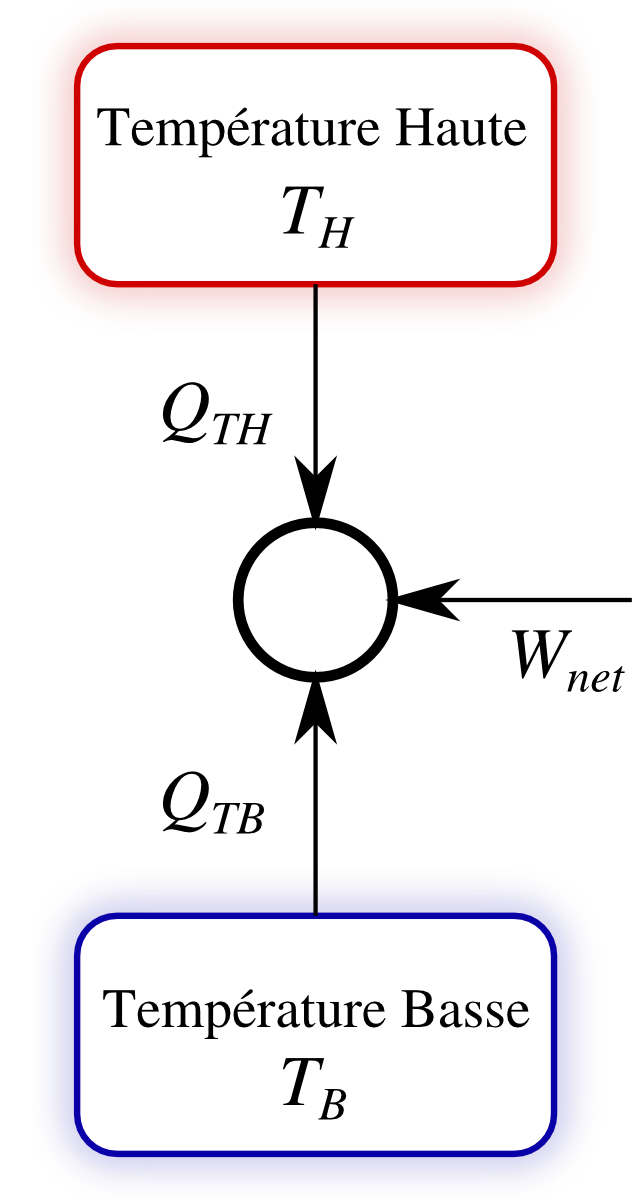
\includegraphics[height=8cm]{images/moteur_forme_generale.png}
		\end{center}
		\caption{Machine thermique transformant travail et chaleur, dans sa représentation la plus générale.}
		\label{fig_conventions_notation_machines_thermiques}
	\end{figure}

	\clearfloats
	Le second principe a des conséquences particulières pour chacun deux grands types de machines thermiques :

	\begin{description}

		\item[Un moteur]{prélève de la chaleur d’une source à haute température ($\dot{Q}_{TH} > 0$) et produit un travail ($\dot{W}_\text{net} < 0$). Nous venons de voir que si l’on veut effectuer cette transformation en continu, nous n’avons d’autre choix que de rejeter de la chaleur dans un réservoir à basse température ($\dot{Q}_{TB} < 0$).

		\begin{figure}
			\begin{center}
				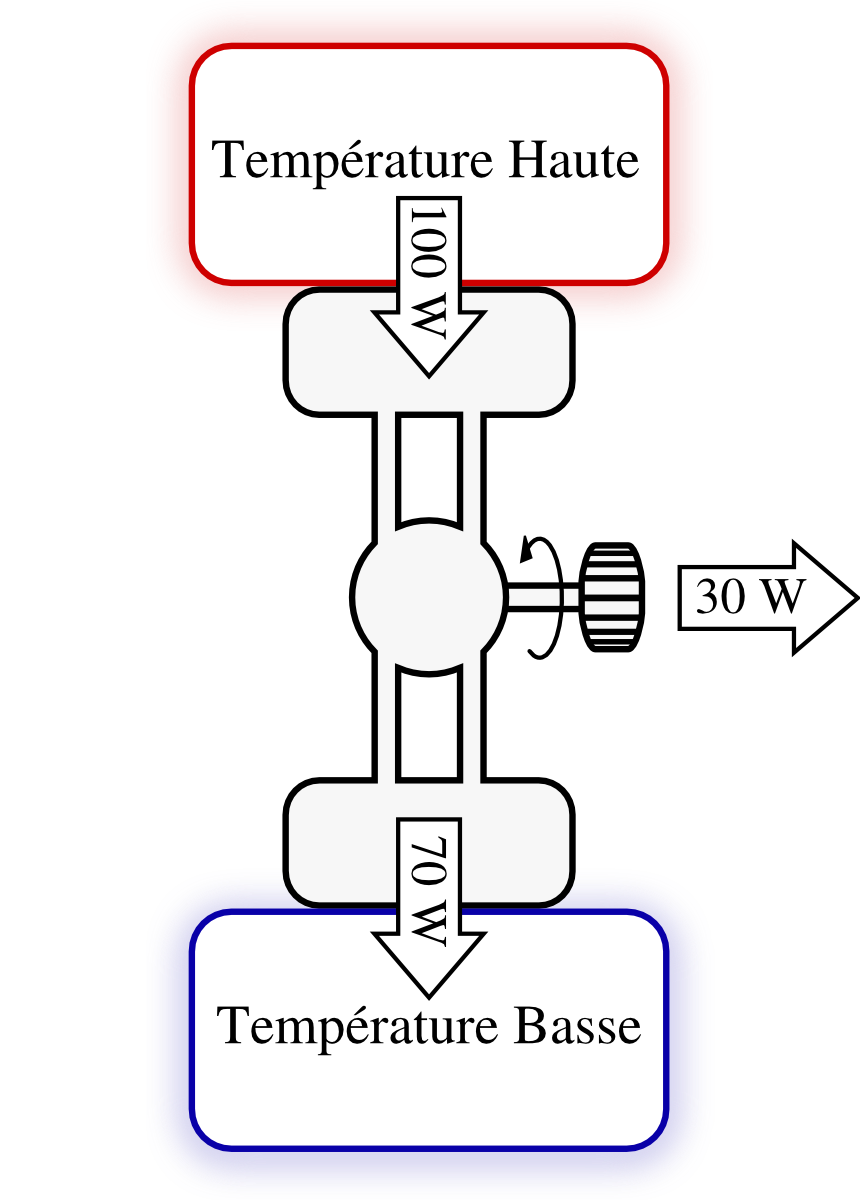
\includegraphics[height=8cm]{images/exemple_moteur.png}
			\end{center}
			\caption{Exemple de moteur.}
		\end{figure}

		Dans les centrales électriques, les deux zones de température sont identifiables facilement : la vapeur prélève de la chaleur au cœur de la centrale (réacteur nucléaire, chaudière à gaz ou à charbon) et rejette de la chaleur par les larges cheminées de refroidissement.

		Les moteurs automobiles et aéronautiques, quant à eux, doivent vidanger l’air qui leur sert de fluide de travail à cause des produits de combustion qui empêchent leur ré-utilisation. Pour cette raison, le refroidissement a lieu dans l’atmosphère, en dehors de la carcasse du moteur. Leur «~zone de refroidissement~» n’est pas distinguable facilement.

		Appliqué au moteur, le second principe peut s’exprimer ainsi :

		\begin{trucimportant}
		Aucun moteur ne peut transformer continûment\linebreak
		de la chaleur en travail\linebreak
		à partir d’une seule source de chaleur.\linebreak
		Tous les moteurs rejettent de la chaleur à plus faible température.\linebreak
		\end{trucimportant}
		\begin{trucimportant}
		Le fonctionnement en continu d’un moteur\linebreak
		nécessite deux réservoirs de chaleur, de température différente.
		\end{trucimportant}

		Les puristes exprimeront ce corollaire, dit \textit{de Kelvin-Planck}, avec l’inéquation suivante :
		\begin{equation}
			\dot{Q}_{TH} > -\dot{W}_\text{net}
		\end{equation}

		\begin{equationterms}
			\item pour tout moteur thermique.
		\end{equationterms}

	}%end item

	\clearfloats
	\item[Un réfrigérateur]{fonctionne dans le sens inverse. Il extrait de la chaleur d’une source à basse température ($\dot{Q}_{TB} > 0$) pour la rejeter dans un réservoir à plus haute température ($\dot{Q}_{TH} < 0$). Une conséquence inévitable est qu’il consomme pour cela du travail ($\dot{W}_\text{net} > 0$).



		\begin{figure}
			\begin{center}
				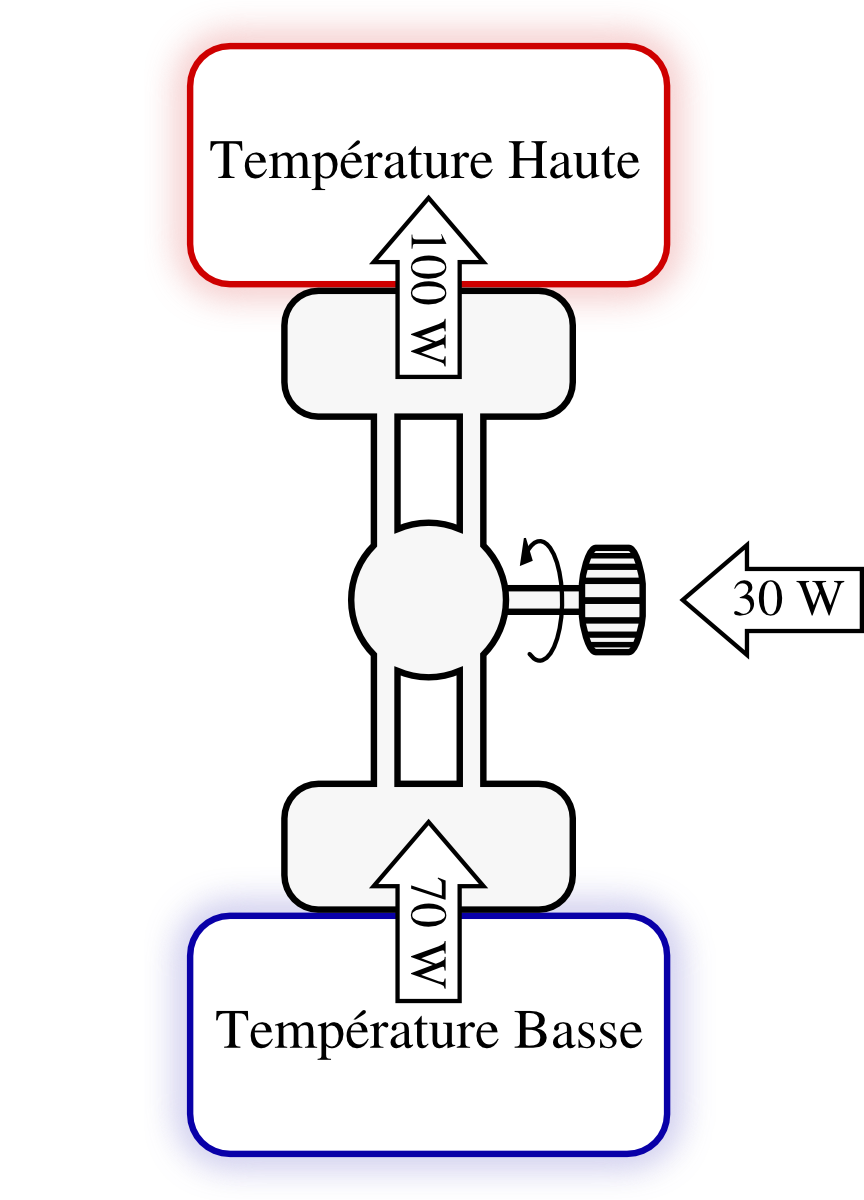
\includegraphics[height=8cm]{images/exemple_refrigerateur.png}
			\end{center}
			\caption{Exemple de réfrigérateur
		(parfois nommé «~machine thermique inversée~»)}
		\end{figure}

		Nous parlons ici de réfrigérateur mais le même principe de fonctionnement s’applique aux climatiseurs ainsi qu’aux pompes à chaleur, comme nous l’avons vu au \courssix.

		Appliquée à un réfrigérateur, la seconde loi s’exprime ainsi :

		\begin{trucimportant}
		Toute machine transférant de la chaleur depuis un corps vers un autre de température plus haute consomme du travail.
		\end{trucimportant}

		Les puristes se plairont à traduire ce corollaire (dit \textit{de Clausius}) ainsi :
		\begin{equation}
			\dot{W}_\text{net réfrigérateur} > 0
		\end{equation}

	}%end item
	\end{description}




\section{Le cycle de Carnot}
\label{ch_cycle_de_carnot}



	\subsection{Un peu d’histoire}

		Au début du \textsc{xix}\ieme siècle, un jeune polytechnicien parisien nommé \wfd{Sadi Carnot (physicien)}{Sadi Carnot} s’est intéressé au fonctionnement des moteurs thermiques dont on assistait alors à la naissance.

		La démarche de Carnot a ceci d’intéressant qu’il a fait entièrement abstraction de l’aspect technologique, pour rechercher les principes sous-jacents des moteurs. C’est d’autant plus difficile qu’à l’époque ceux-ci fonctionnent en utilisant l’ébullition et la condensation de la vapeur, et que la notion de \emph{cycle} n’était pas encore acquise --\ pas plus que la notion de conservation de l’énergie.

		Carnot recherchait \emph{la quantité maximale de travail} qu’il est possible de générer à partir d’une quantité donnée de charbon. Ses travaux (\textit{Réflexions sur la puissance motrice du feu et sur les machines propres à développer cette puissance}, 1824) n’ont jamais été reconnus de son vivant ; sa conception de la chaleur était profondément erronée%
			\footnote{Il s’agit encore et toujours de la \wfd{Théorie du calorique}{théorie du \vocab{calorique}}, due à \wfd{Antoine Lavoisier}{Lavoisier}, qui sera démontée brique par brique par \we{James Prescott Joule} ; mais il faudra attendre encore vingt années…}%
		 ; et pourtant, le moteur théorique qu’il a décrit, passage incontournable pour l’étudiant/e en ingénierie, sert de référence dans les bureaux d’études de tous les motoristes aujourd’hui.



	\subsection{Concept de machine réversible}

		Carnot recherche le moteur théorique dont l’efficacité est maximale. Il imagine une façon unique de transformer chaleur en travail, et travail en chaleur. Sa machine peut fonctionner dans les deux sens : en tant que moteur ou bien en tant que réfrigérateur.

		En termes thermodynamiques, le moteur qu’il conceptualise est \vocab{réversible}. En inversant son fonctionnement, tous les flux de chaleur seront inversés. De cette façon, si son réfrigérateur est alimenté par son moteur, alors les flux seront compensés, comme représenté en \cref{fig_deux_machines_de_carnot}.

		\begin{figure}
			\begin{center}
				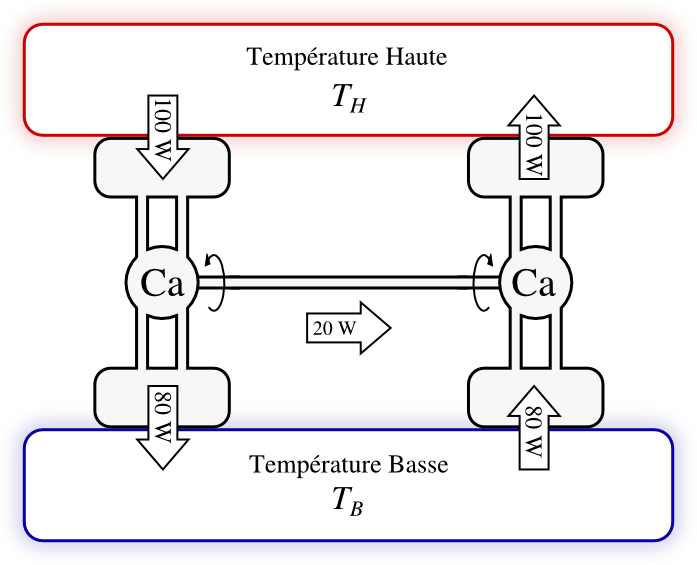
\includegraphics[height=8cm]{images/carnot_moteur_refrigerateur.png}
			\end{center}
			\caption{Deux machines de Carnot, un moteur (à gauche) et un réfrigérateur (à droite).
			La première alimente la seconde, et comme elles sont réversibles, les flux de chaleur sont compensés.}
			\label{fig_deux_machines_de_carnot}
		\end{figure}

		Pourquoi une telle machine serait-elle la plus efficace que l’on puisse concevoir ?

		On peut montrer par l’absurde qu’un moteur ayant une efficacité supérieure à un moteur réversible ne peut exister (\cref{fig_plus_que_machine_de_carnot}). Le travail fourni par cette machine hypothétique pourrait être utilisé pour alimenter un réfrigérateur réversible. Ces deux machines réunies, ensemble, ne consommeraient alors aucun travail, mais provoqueraient tout de même un flux de chaleur depuis le réservoir froid vers le réservoir chaud. Selon Carnot, et d’après le second principe dont nous avons admis la validité, c’est impossible.

		\begin{figure}
			\begin{center}
				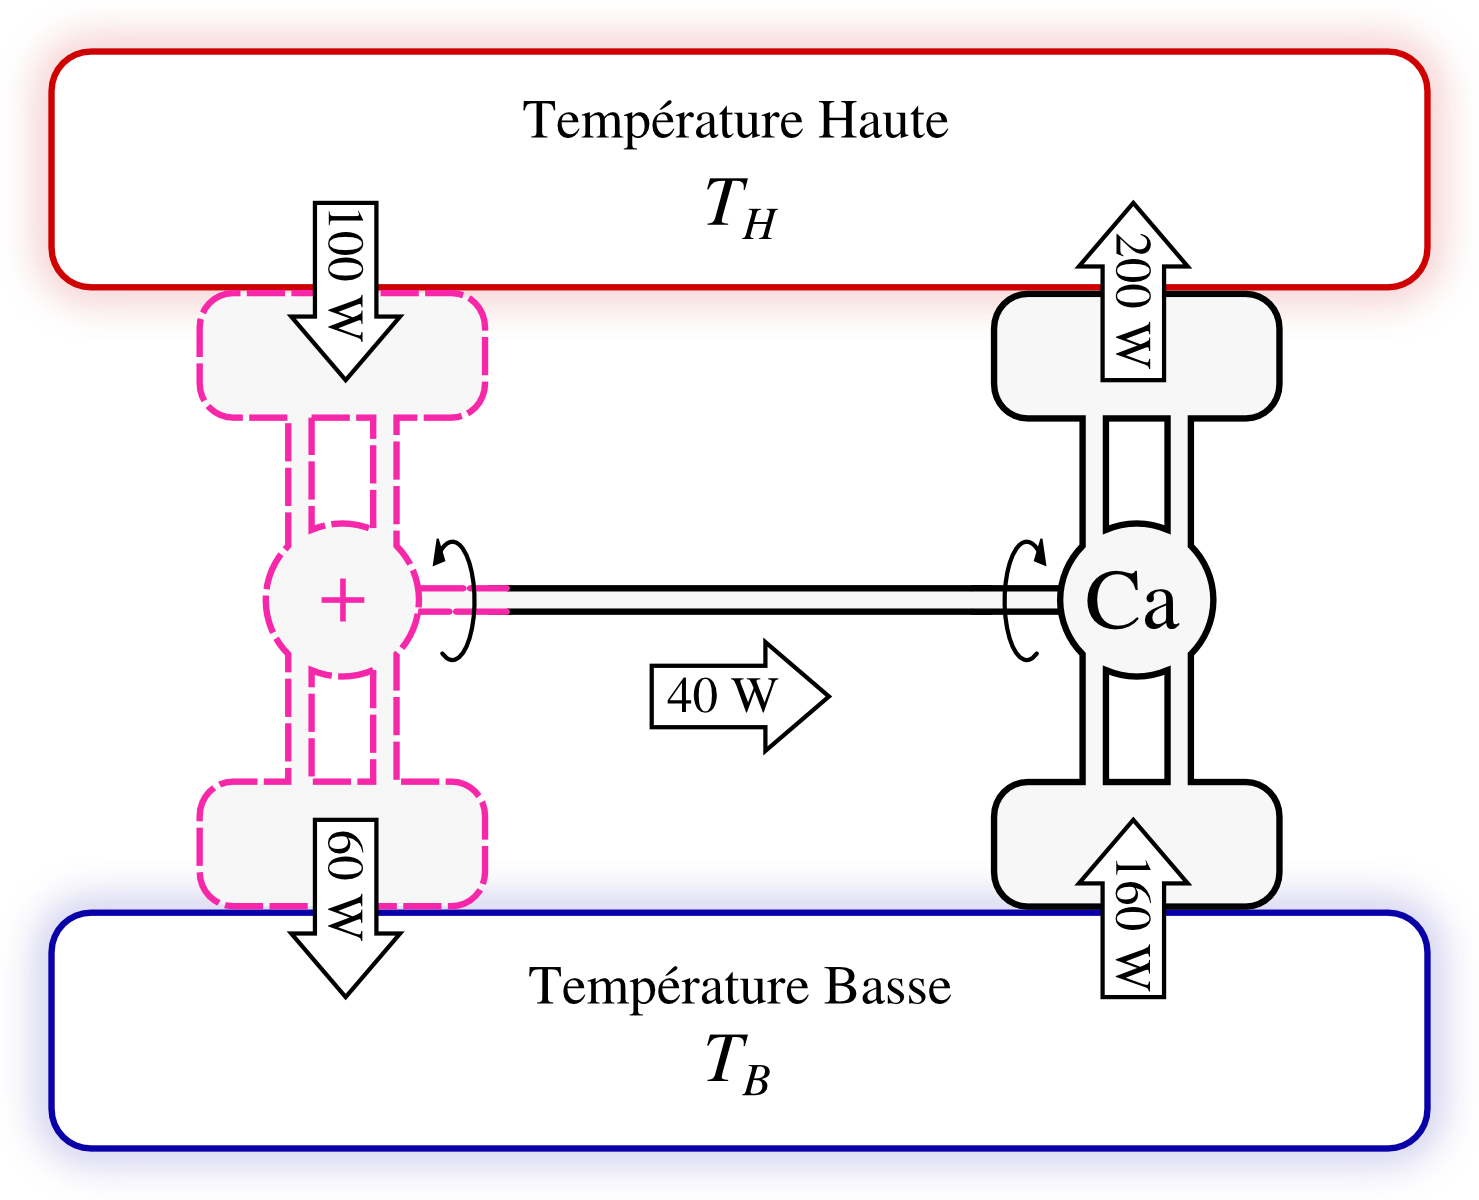
\includegraphics[height=8cm]{images/carnot_moteur_plusplus.png}
			\end{center}
			\caption{Démonstration par l’absurde du fait que le meilleur moteur possible est réversible.
		Un hypothétique moteur irréversible (à gauche) qui aurait une plus grande efficacité qu’un réfrigérateur réversible (à droite) pourrait simplement alimenter ce dernier. Ainsi, on obtiendrait un flux net spontané de chaleur (de~\SI{100}{W}) depuis la source froide vers la source chaude, sans apport net de travail : selon le second principe, c’est impossible.}
			\label{fig_plus_que_machine_de_carnot}
		\end{figure}

		Cette méthode de raisonnement par combinaison de machines hypothétiques et théoriques, même s’il peut dérouter, est une excellente façon d’approcher la théorie des moteurs. L’étudiant/e est vivement encouragé/e à expérimenter ainsi, en se posant par exemple les questions suivantes :

		\begin{itemize}
			\item Pourquoi le meilleur réfrigérateur possible fonctionne-t-il de façon réversible ?
			\item Peut-on améliorer un moteur en ré-injectant ses rejets de chaleur à la source chaude à l’aide d’une pompe à chaleur réversible ?
		\end{itemize}



	\subsection{Clés du fonctionnement de la machine de Carnot}

		L’efficacité maximale est donc obtenue avec une machine réversible. À partir de ce constat, Carnot raisonne de la façon suivante :

		\begin{enumerate}
			\item Un moteur thermique fonctionne avec la dilatation et la contraction d’un corps soumis alternativement à deux températures ;
			\item Pour qu’ils soient réversibles, c’est-à-dire pour pouvoir être effectués dans le sens inverse, tous les échanges de chaleur doivent être effectués avec des différences de température infinitésimales : ces transformations seront alors \emph{isothermes} ;
			\item Pour qu’elles soient réversibles, les phases où le corps change de température (pour passer d’un réservoir de chaleur à un autre) doivent se faire sans échange de chaleur : ces transformations seront alors \emph{adiabatiques}.
			\item Pour permettre un retour en arrière avec chaque évolution, il faut qu’elles soient toutes \emph{réversibles} (infiniment lentes).
		\end{enumerate}

		L’essentiel est dit. Carnot vient ici de dessiner un cycle thermodynamique théorique, composé de deux évolutions isothermes et deux évolutions adiabatiques. Il n’a pas eu besoin de quantifier le moindre transfert ; et ne s’est pas encore soucié du moindre détail technologique. Pourtant, il est certain que le cycle thermodynamique qu’il décrit est le plus efficace --\ le moins inefficace !\ -- qu’il soit possible d’effectuer.

		 

	\subsection{Fonctionnement du moteur de Carnot}
	\label{ch_descritpion_cycle_carnot}

		Il est possible de décrire le \vocab{cycle de Carnot} avec un système piston-cylindre\footnote{Il est également possible de décrire ce cycle avec un système turbine-compresseur fonctionnant en régime permanent, mais l’évolution est moins intuitive visuellement.} que l’on peut alternativement isoler ou mettre en contact avec les sources chaude et froide. Le cycle comporte quatre étapes réversibles
		\footnote{Il ne faut pas confondre ces quatre étapes avec les quatre temps du moteur à explosion usuel. En théorie, ces quatre étapes sont réalisables avec deux temps (compression, détente) seulement.} %
		et le fluide oscille entre les températures $T_H$ (source «~chaude~» à haute température) et $T_B$ (source «~froide~» à basse température).

		\begin{itemize}

			%renewing bullet as an image at every \item. Quite a lousy hack, no doubt.
			\renewcommand\labelitemi{
\includegraphics[width=3cm]{images/illustration_adiabatique.png}}
			\renewcommand\itemsep{1cm}
			\renewcommand\topsep{3cm}

			\item \textbf{Compression adiabatique réversible de 1 à 2}

		Le cycle débute en 1, lorsque le fluide est dans le cylindre à température basse $T_B$. 

		Pour l’amener à température haute (et ainsi permettre un transfert de chaleur réversible en phase $2\to3$), le fluide est compressé de façon adiabatique réversible\footnote{Les compressions et détentes adiabatiques réversibles sont détaillées aux sections \S\ref{ch_gp_isentropiques} et \S\ref{ch_lv_isentropiques}}.
		La température du fluide augmente de $T_B$ à $T_H$.

		Cette phase est \emph{consommatrice} de travail ($W_{1 \to 2} > 0$). Le but de l’évolution est d’amener le fluide à haute température.

			% again
			\renewcommand\labelitemi{
\includegraphics[width=3cm]{images/illustration_th.png}}
			\item \textbf{Chauffage isotherme de 2 à 3}

		En 2, le fluide se trouve donc compressé dans le piston, à la température $T_H$. 

		Le cylindre alors est mis au contact de la source chaude (température $T_H$) et on fournit de la chaleur avec une différence de température infinitésimale : c’est une détente isotherme\footnote{Les échanges de chaleur isothermes sont détaillés aux sections \S\ref{ch_gp_isothermes} et \S\ref{ch_lv_isothermes}}.

		Cette phase est productrice de travail ($W_{2 \to 3} < 0$). Le but de l’évolution est de capter de la chaleur (quantité $Q_{TH}$) de la source chaude.

			% again
			\renewcommand\labelitemi{
\includegraphics[width=3cm]{images/illustration_adiabatique.png}}
			\item \textbf{Détente adiabatique de 3 à 4}

		Le transfert de chaleur isotherme ci-dessus est stoppé en 3.

		Le cylindre est alors isolé thermiquement. Le but est désormais de réduire la température du fluide jusqu’à $T_{B}$ en produisant le maximum de travail. Pour cela une détente adiabatique réversible a lieu : le piston poursuit son recul infiniment lent, et cette fois le fluide voit sa température descendre progressivement.

		Cette phase est productrice de travail ($W_{3 \to 4} < 0$).

			% one last time
			\renewcommand\labelitemi{
\includegraphics[width=3cm]{images/illustration_tb.png}}
			\item \textbf{Refroidissement isotherme de 4 à~1}

		En 4, le fluide est à température basse $T_{TB}$. 

		Pour le ramener à son volume initial, il faut lui retirer de la chaleur. Pour cela un refroidissement isotherme a lieu ; le piston est avancé progressivement, et la température du fluide est maintenue constante à  $T_{TB}$.

		Cette phase est \textit{consommatrice} de travail ($W_{4 \to 1} > 0$) ; la chaleur rejetée par le fluide vers la source froide est $Q_{TB}$. 

		\end{itemize}

		Au final, le moteur a reçu une quantité de chaleur $|Q_{TH}|$ à haute température, et rejeté une quantité $|Q_{TB}|$ plus faible à basse température. La différence entre ces deux quantités est le travail produit, $|W_\text{net}|$.%
			\footnote{Nous avons bien sûr $W_\text{net} = W_{1 \to 2} + W_{2 \to 3} + W_{3 \to 4} + W_{4 \to 1} = - (Q_{TH} + Q_{TB})$ (\ref{def_travail_net}).}
		Parce que le cycle est réversible, $|W_\text{net}|$ est le maximum qu’il soit possible d’obtenir.

		\begin{landscape}

		\begin{figure}
			\begin{center}
				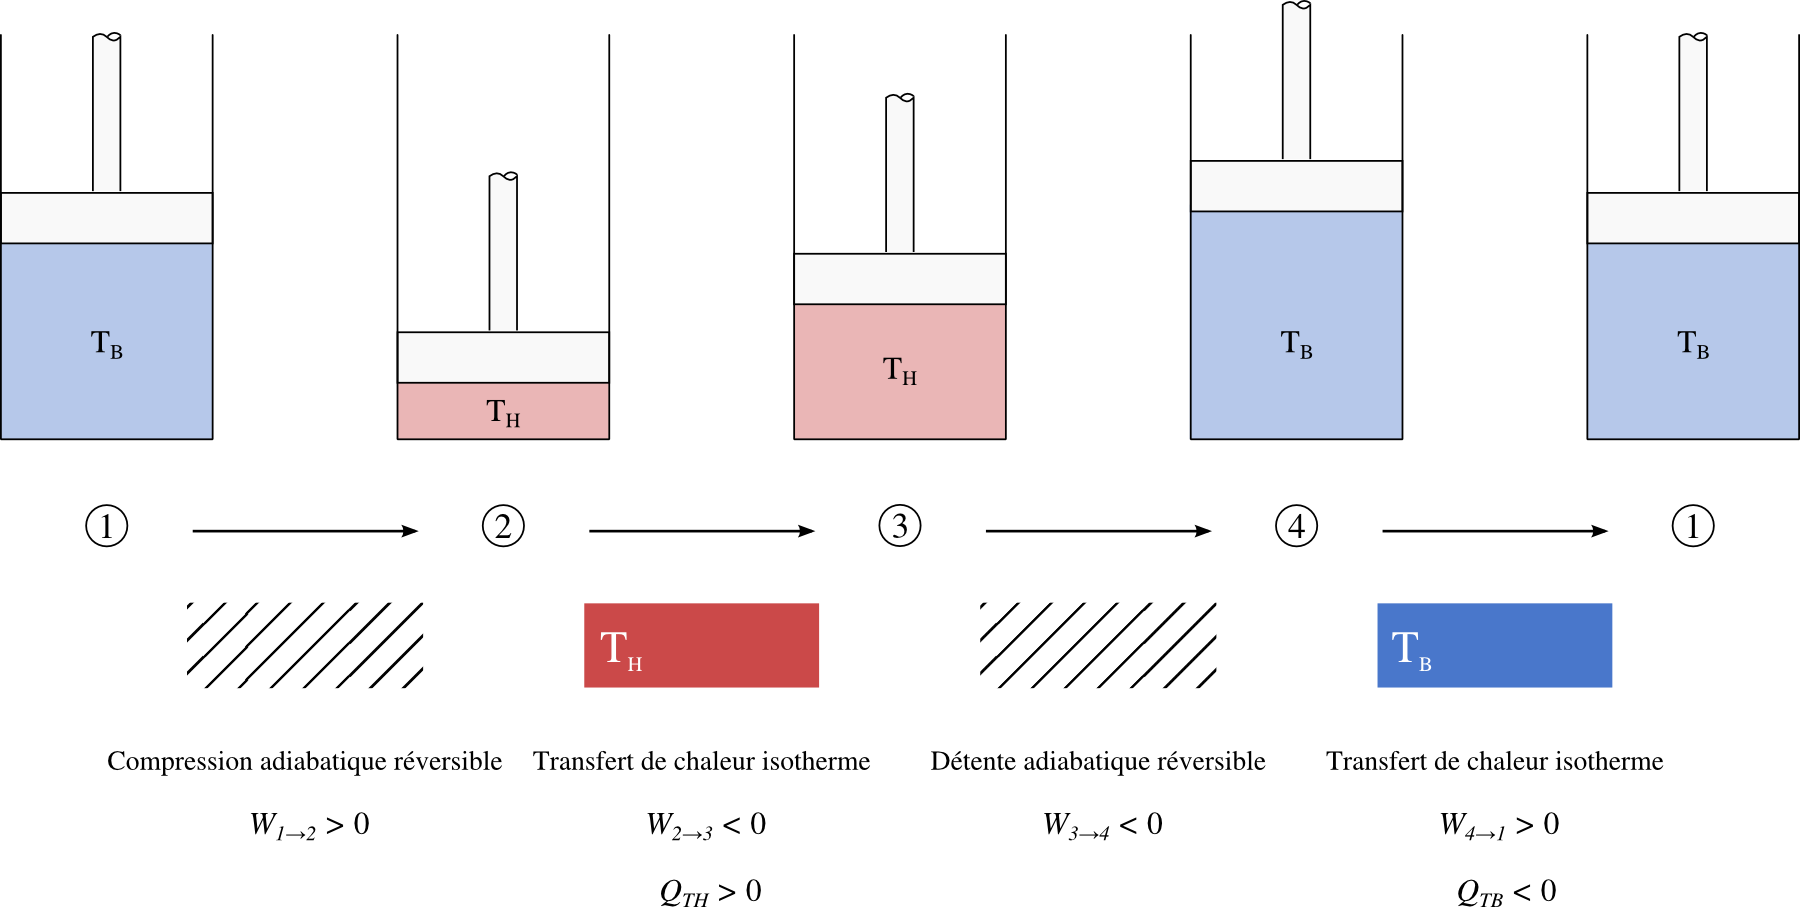
\includegraphics[width=\linewidth]{images/carnot_description_complete.png}
			\end{center}
			\caption{Les quatre étapes du moteur de Carnot.}
			\label{fig_carnot_quatre_etapes}
		\end{figure}

		\end{landscape}

		Le cycle du moteur de Carnot peut être tracé sur un diagramme pression-volume (comme par exemple en \cref{fig_p-v_gp_carnot} avec un gaz parfait). On observe notamment que les phases de compression se font à plus basses pression et volume que les phases de détente : le cycle est producteur de travail. L’aire circonscrite dans le parcours 1-2-3-4-1 représente la quantité de travail produite.

		Le fait qu’aucune de ces étapes ne soit réalisable en pratique n’aura pas échappé à l’étudiant/e perspicace : pour que toutes ces phases soient réversibles, il faut que le mouvement du piston soit infiniment lent.

		\begin{figure}[htp] %handmade
			\begin{center}
				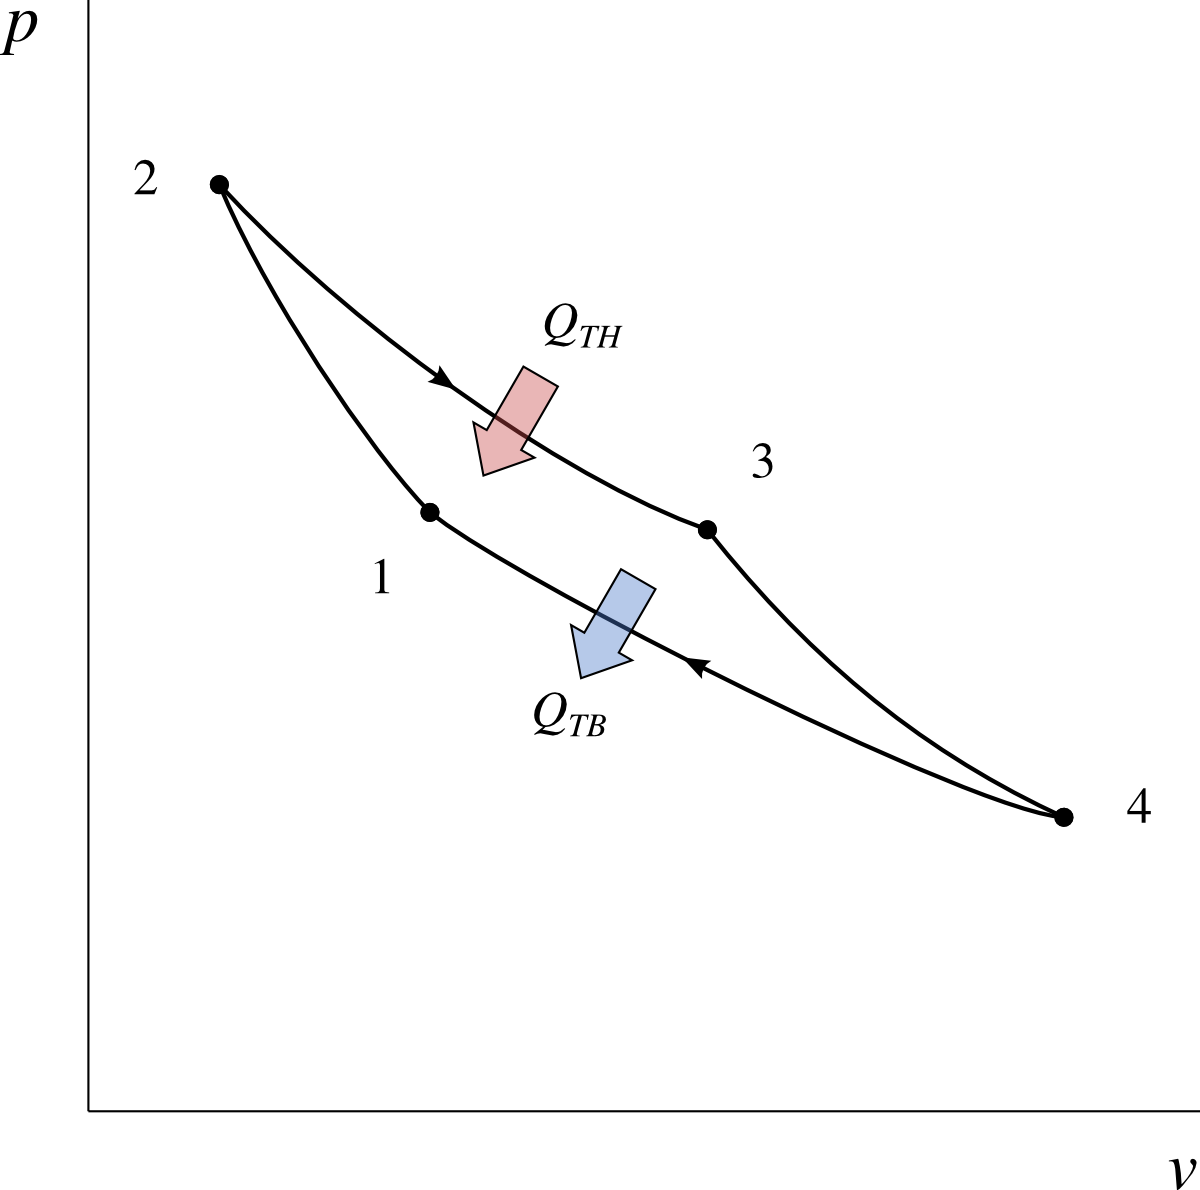
\includegraphics[width=10cm]{images/carnot_pv_gp_moteur.png}
			\end{center}
			\caption{Diagramme pression-volume d’un cycle de Carnot, pour un moteur, avec un gaz parfait. Dans le cas d’une machine thermique inversée (réfrigérateur ou pompe à chaleur), le sens de l’évolution est simplement inversé.}
			\label{fig_p-v_gp_carnot}
		\end{figure}



	\subsection{Le réfrigérateur de Carnot}

		En inversant le sens de fonctionnement, on crée un système de réfrigération de même efficacité. Le fluide passe alors par les mêmes états, mais en parcourant le chemin inverse (1-4-3-2-1) comme montré en \cref{fig_p-v_gp_carnot_inversé}. La chaleur $|Q_{TB}|$ est \emph{captée} de la source froide, le travail $|W_\text{net}|$ est \textit{reçu} par la machine, et la chaleur $|Q_{TH}|$ est rejetée par la machine vers la source à haute température.

		Ce cycle permet d’obtenir le rendement maximal (le moins mauvais rendement, car il n’est pas infini) d’un système de climatisation ou d’une pompe à chaleur.

		\begin{figure}
			\begin{center}
				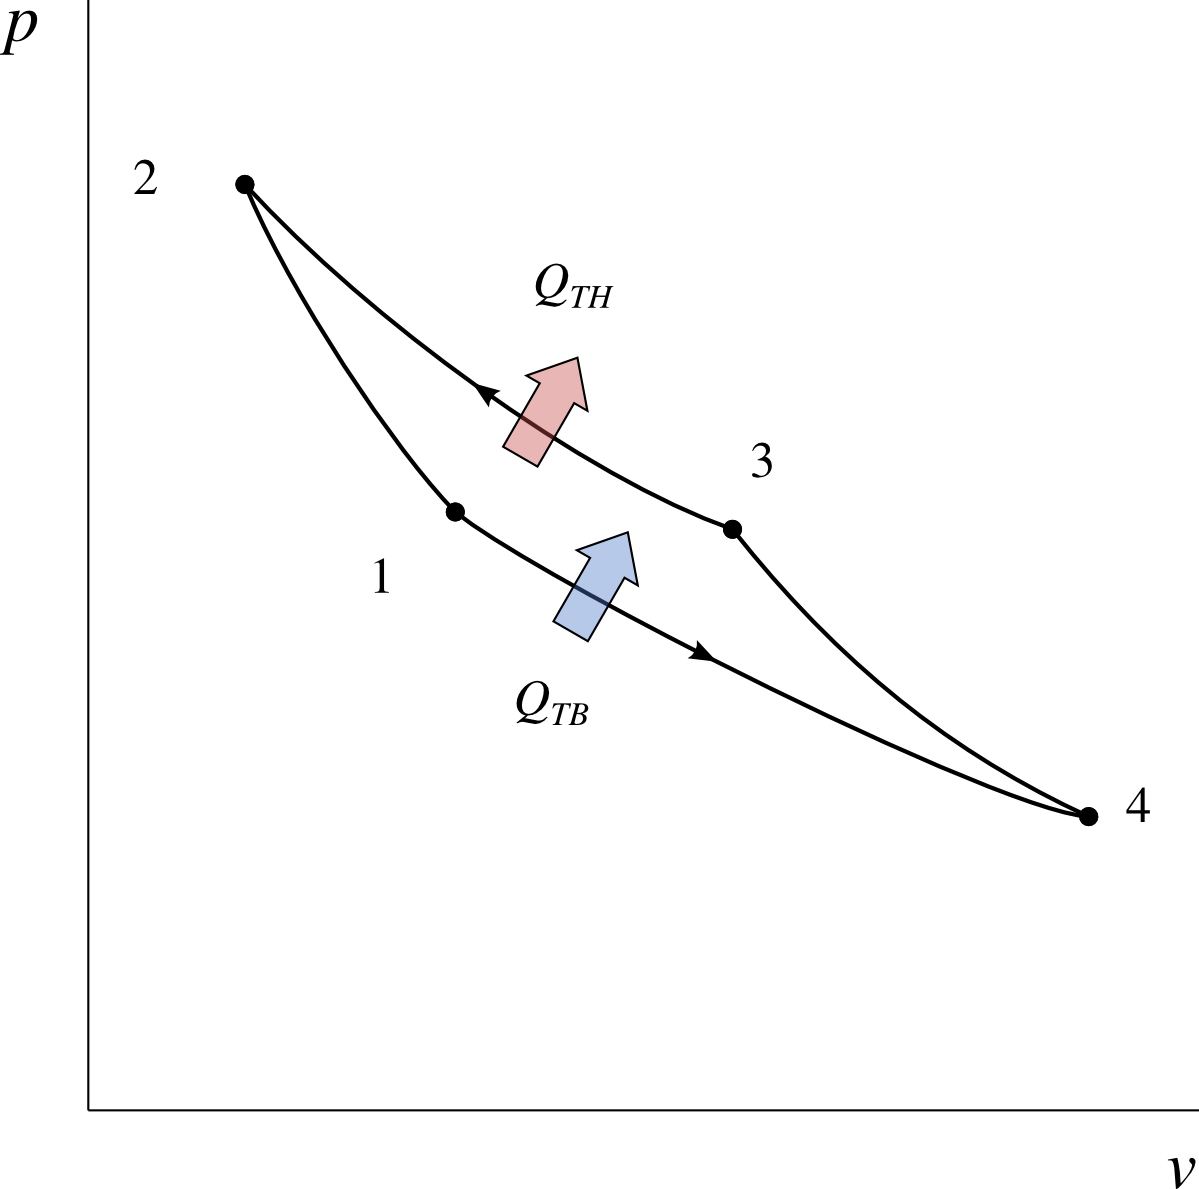
\includegraphics[width=10cm]{images/carnot_pv_gp_refrigerateur.png}
			\end{center}
			\caption{Diagramme pression-volume pour un cycle de Carnot inversé, c’est-à-dire en mode de réfrigération (réfrigérateur ou pompe à chaleur), avec un gaz parfait.}
			\label{fig_p-v_gp_carnot_inversé}
		\end{figure}





\section{L’échelle de température thermodynamique}


	\subsection{L’essentiel à retenir}
	
		Kelvin définit une échelle de température, dite de \vocab{température absolue}. À l’intérieur d’une machine de Carnot, le rapport des températures maximale $T_H$ et minimale $T_B$ est défini comme égal au rapport des débits sous forme de chaleur, c’est-à-dire :
			
		\begin{equation}
			\left| \frac{\dot{Q}_{TH}}{\dot{Q}_{TB}} \right| \equiv  \frac{T_H}{T_\B } \tag{\ref{def_échelle_température_kelvin}}
		\end{equation}
		
		\begin{equationterms}
			\item par définition, dans une machine de Carnot,
			\item où \tab $\dot{Q}_{TH}$ \tab est le débit de chaleur absorbé ou rejeté à haute température ($\dot{Q}_{TB}$, à basse température),
			\item et où les températures sont absolues (mesurées en \si{\kelvin}).
		\end{equationterms}

		Cette \cref{def_échelle_température_kelvin} est une définition. On peut donc déterminer la température d’un corps sans devoir utiliser un fluide en particulier. Kelvin étalonne son échelle de sorte que $\SI{0}{\degreeCelsius} = \SI{273,15}{\kelvin}$. 
		
		Les paragraphes qui suivent sont destinés aux lecteurs curieux, et peuvent être survolés sans danger par l’étudiant/e ou l’ingénieur/e pressé/e. 

	\subsection{Qu’est-ce qu’une échelle en physique ?}
	
		Pour quantifier une propriété en physique (par exemple, quantifier «~la masse~» ou «~la couleur~»), il faut avoir défini trois choses :
		
		\begin{description}
			\item [Un degré zéro] qui définit ce que représente zéro propriété (zéro masse, zéro longueur, etc.) ;
			\item [Un étalon] arbitraire qui sert de calibre (par exemple, un objet de masse une livre, de longueur un mètre) ;
			\item [Une échelle] qui permet de définir la propriété entre le degré zéro et l’étalon (par exemple, ce qu’est «~deux fois plus~» ou «~deux fois moins~» de masse, de lumière, etc.).
		\end{description}
	
	\subsection{Les limites des thermomètres de Celsius et Fahrenheit}
	
		Au début du \textsc{xix}\ieme siècle, les deux échelles de température que nous utilisons aujourd’hui dans la vie courante, celles du suédois \wf{Anders Celsius} et de l’allemand \wf{Gabriel Fahrenheit}, sont déjà en usage. Qu’en est-il de ces deux échelles d’un point de vue physique ?
			
		\begin{itemize}
			\item Le degré zéro est plutôt facile à définir (c’est le point où les corps sont entièrement figés, incapables de fournir de la chaleur) mais ni Fahrenheit ni Celsius ne sont capables de le situer avec certitude ;
			\item Les étalons de Celsius et Fahrenheit sont sensiblement différents. Celsius choisit le gel de l’eau pure, Fahrenheit de l’eau salée, à pression atmosphérique, et lui attribuent chacun la graduation relative «~zéro~».
			\item Les échelles de Celsius et Fahrenheit, en revanche, sont strictement identiques. En effet, pour \emph{mesurer} les températures autour de leurs étalons, les deux scientifiques mesurent la contraction et la dilatation d’un liquide dans un tube. Entre son zéro et l’ébullition de l’eau à pression atmosphérique, Celsius trace 100 graduations%
			\footnote{En fait, Celsius utilise initialement une échelle inversée, allant de~\SI{100}{\celsius} au gel jusqu’à~\SI{0}{\celsius} à l’ébullition !} ; Fahrenheit, 212 graduations%
			\footnote{Cette graduation est probablement choisie pour se recaler facilement sur sa \emph{première} graduation, étalonnée sur le gel de l’eau pure (32) et la température du corps humain (96). Des étalons fort difficiles à reproduire !}.
		\end{itemize}
		
		Le principal problème avec ces deux échelles est que la température n’est bien définie que dans le domaine d’existence des thermomètres à liquide. Quel que soit le fluide utilisé (mercure, alcool, eau), il finit toujours par geler ou bouillir quelque part ; et les graduations ne donnent alors plus d’information utile. Par exemple, Celsius ne peut pas \emph{définir} ou même décrire ce qui permet de reconnaître une température de~\SI{1200}{\celsius}.
		
		En plus de cela, les deux échelles sont peu intuitives à utiliser en dessous du gel de l’eau. Pour peu que l’on admette, par exemple, que \SI{40}{\celsius} puisse être «~deux fois plus de température~» que \SI{20}{\celsius}, alors à quoi correspondrait une température deux fois plus haute que \SI{-10}{\celsius} ?\footnote{Cela revient à poser la question : peut-on écrire $\frac{\SI{40}{\celsius}}{\SI{20}{\celsius}}$ et est-ce égal à $\frac{\SI{80}{\celsius}}{\SI{40}{\celsius}}$ ? (la réponse moderne à cette question est non.)}
		
		
	
	\subsection{Le thermomètre de William Thomson}
	
		\wfd{William Thomson (Lord Kelvin)}{William Thomson}, ingénieur et physicien écossais, a bien compris ces limites. Il va proposer une échelle de température qui, elle, ne dépend pas du comportement d’un fluide dans un tube.

		Thomson s’intéresse de près au cycle de Carnot et il raisonne de la façon suivante. La seule propriété qui confère l’efficacité maximale au moteur de Carnot est le fait qu’il soit réversible. Autrement dit, toutes les machines fondées sur ce cycle et opérant entre deux températures données auront la même efficacité —\ quels que soient leur carburant, leur cylindrée, leur configuration, ou leur puissance\footnote{On pourrait par exemple «~allonger~» tant qu’on veut les phases de détente isotherme : rien ne fixe \textit{a~priori} l’état 3 décrit en \cref{fig_carnot_quatre_etapes}).}. On pourrait donc se servir de l’efficacité d’un moteur de Carnot comme mesure de la température.
		
		La proposition de Thomson est la suivante : soit un corps à une température $T_1$ (par exemple de mille unités, comme montré en \cref{fig_échelle_température_kelvin}). On y attache un moteur de Carnot, qui va fournir du travail et rejeter de la chaleur à température plus basse $T_2$. Cette température $T_2$ est deux fois plus faible que $T_1$ si le moteur rejette la moitié de la chaleur qu’il reçoit ; elle est quatre fois plus faible lorsqu’il en rejette le quart, etc. En termes mathématiques, Thomson propose\footnote{En fait, ce n’est pas si simple. Thomson propose d’abord (en 1848) une échelle dans laquelle $\frac{\dot{Q}_{TH}}{\dot{Q}_{TB}}$ est proportionnel à la \emph{différence} des températures ; ce qui en fait une échelle logarithmique de notre point de vue actuel. Il se ravise avec la proposition~\ref{def_échelle_température_kelvin} six ans plus tard.} :
			
		\begin{equation}
			\left| \frac{\dot{Q}_{TH}}{\dot{Q}_{TB}} \right| \equiv  \frac{T_H}{T_\B }
			\label{def_échelle_température_kelvin}
		\end{equation}

		\begin{equationterms}
			\item dans une machine de Carnot (en fait, pour toute machine effectuant une transformation réversible),
			\item où \tab $\dot{Q}_{TH}$ \tab est le débit de chaleur absorbé ou rejeté à haute température ($\dot{Q}_{TB}$, à basse température),
			\item et où les températures sont \vocab{absolues} (mesurées en \si{\kelvin}).
		\end{equationterms}

		\begin{figure}
			\begin{center}
				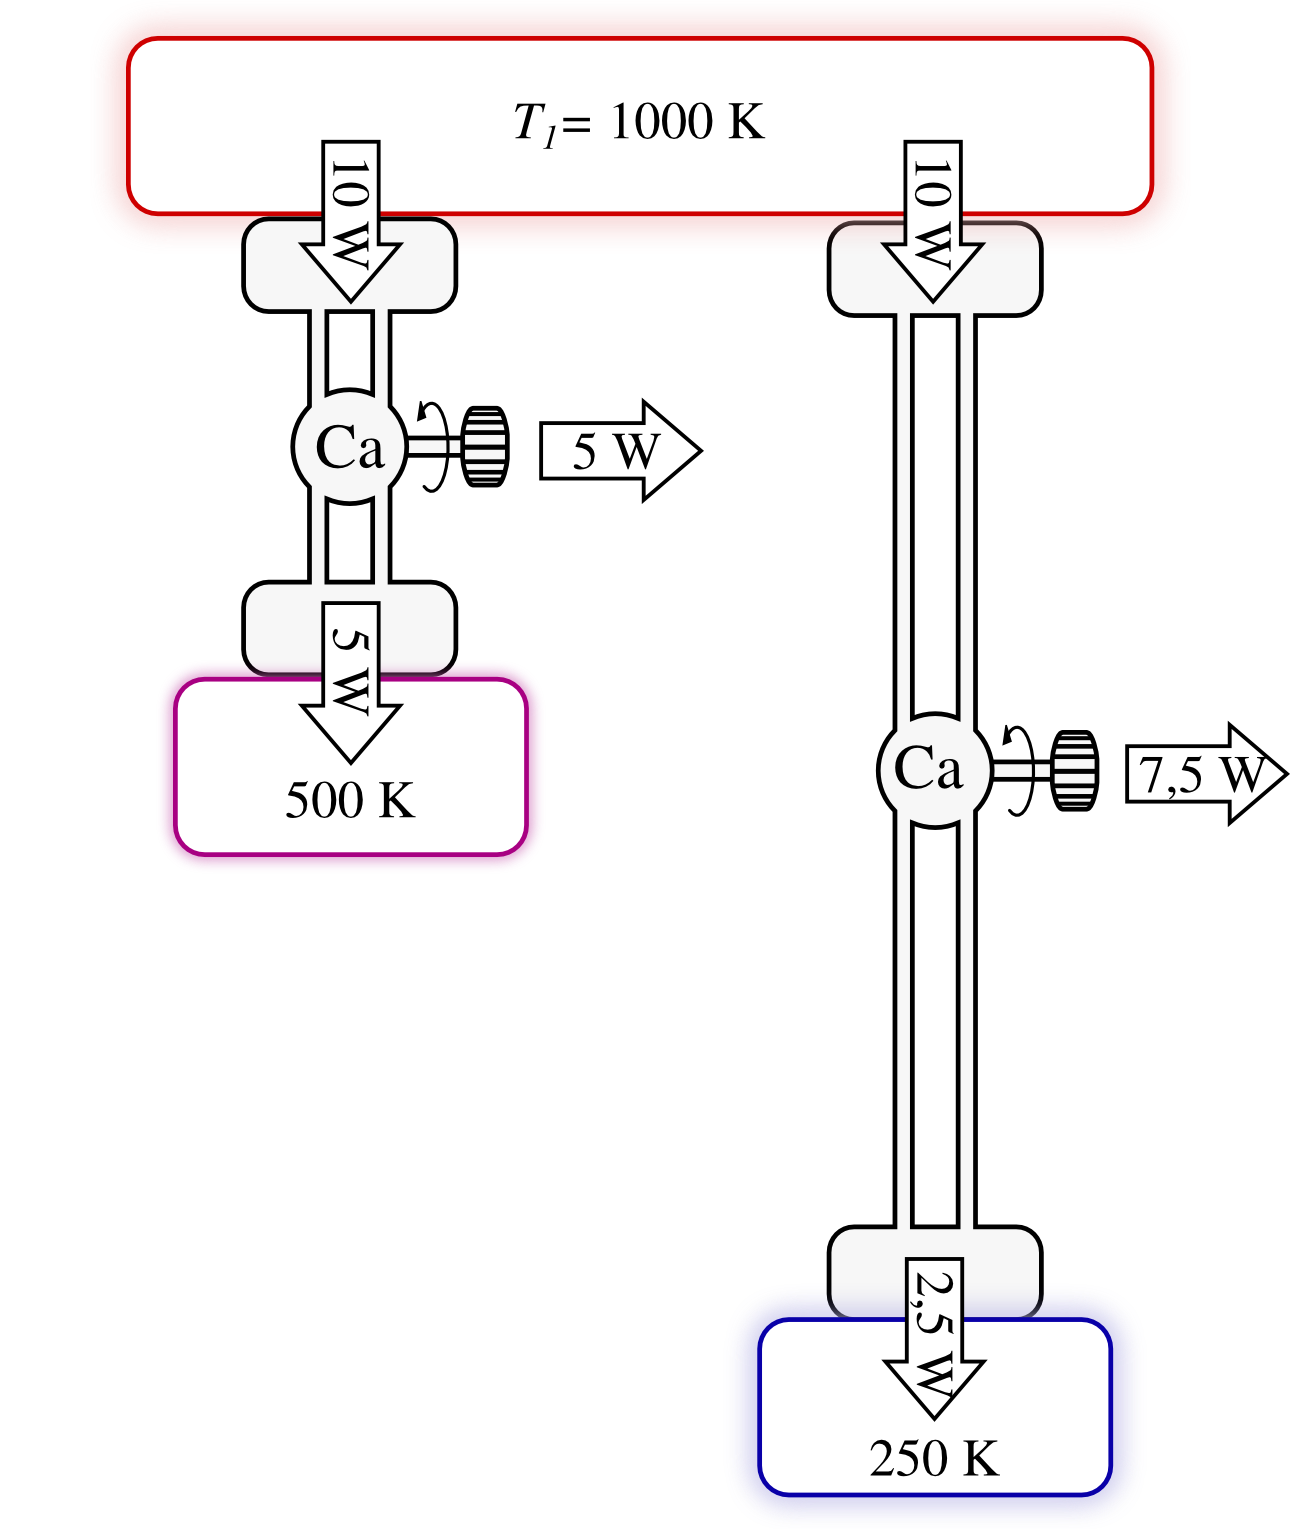
\includegraphics[width=10cm]{images/echelle_temperature_kelvin.png}
			\end{center}
			\supercaption{Expérience permettant d’illustrer l’échelle de température absolue proposée par William Thomson. Un moteur de Carnot fonctionnant entre \SI{1000}{\kelvin} et~\SI{500}{\kelvin} rejette $\frac{\num{1000}}{\num{500}} = \SI{50}{\percent}$ de la chaleur qu’il reçoit. Si la température basse est quatre fois plus faible, ce rejet est quatre fois plus faible ($\frac{\num{1000}}{\num{250}}$) que la chaleur reçue.}{}
			\label{fig_échelle_température_kelvin}
		\end{figure}


		Avec une simple manipulation des équations~\ref{def_échelle_température_kelvin} et~\ref{eq_premier_principe_machines}, on peut reformuler la définition de Kelvin comme suit :

		\begin{trucimportant}
		Soit une machine de Carnot fonctionnant 
		entre deux réservoirs thermiques séparés d’un degré de température (\SI{1}{\kelvin}),\linebreak
		et à laquelle on fournit une quantité de chaleur $Q_{H}$ de~\SI{1}{Joule} ;

		La température de la source chaude\linebreak est définie comme l’inverse du travail produit.
		\end{trucimportant}

		
		Les températures dans cette échelle, dite \vocab{échelle de température absolue} ou \vocab{de température thermodynamique}, sont toujours positives et varient de zéro à l’infini. 
				
	\subsection{Zéro absolu et synchronisation des échelles}
	
		Thomson dispose donc d’une \vocab{échelle} —\ une méthode permettant de définir une température «~deux fois plus élevée~».
		
		Le zéro de cette échelle correspond bien au degré zéro de température, puisqu’avec l’expérience de la \cref{fig_échelle_température_kelvin} on dispose alors d’un «~gouffre~» de température zéro qui permet de détendre les gaz jusqu’à zéro température (on peut ainsi convertir toute l’énergie interne d’un fluide en travail\footnote{On peut prendre une machine de Carnot avec $T_\B = \SI{0}{\kelvin}$. Le transfert de chaleur à la source froide est alors inutile puisque l’on a effectué une détente infinie ($3 \to 4$) pour obtenir une température de zéro. $Q_{TB}$ est alors nul, et on retrouve bien un rendement de~\SI{100}{\percent}.}).
		
		Reste le choix d’un étalon. Thomson revient au thermomètre de Celsius et prend le même point de référence (gel de l’eau à pression atmosphérique). Observant que la contraction et la dilatation des fluides reste proportionnelle à leur variation de température absolue, il attribue à ce point de référence une valeur qui permet de conserver la même graduation thermométrique. Pour cela, il faut que les températures \SI{100}{\celsius} et~\SI{0}{\celsius}, dont on sait qu’elles permettent un rendement maximal de~\SI{28,8}{\percent}, correspondent à des températures en \si{\kelvin} espacées de 100 unités. Le calcul est simple\footnote{L’étudiant/e est encouragé/e à le reproduire.} et Thomson obtient la relation :
			
			\begin{equation}
			\SI{0}{\degreeCelsius} = \SI{273,15}{\kelvin}
			\label{eq_synchro_température}
			\end{equation}
		
		William Thomson a trente ans lorsqu’il publie son échelle de température en 1854, lancé dans une carrière de scientifique époustouflante. En 1892 il sera sacré \textit{Premier Baron Kelvin}\footnote{On dira même \textit{The Right Honourable First Lord Kelvin (OM, GCVO, PC, PRS, PRSE)} !} ; c’est sous ce nom qu’il est connu aujourd’hui. L’unité \textit{Kelvin} (\si{\kelvin}) est officiellement attribuée à la température absolue en 1948. 
		
		Le travail de Kelvin permet donc de séparer définitivement le concept de température des fluides réels ou imaginaires (ébullition de l’eau, volume des gaz parfaits\footnote{Nous avions esquivé deux fois la définition de la température dans ces chapitres (\S\ref{ch_définition_température_cours1} et \S\ref{ch_le_manomètre_comme_thermomètre}).}) ; la voilà rattachée à une expérience physique précise et quantitative.
		






\section{Efficacité maximale des machines}

		La définition de la température détaillée en~\ref{def_échelle_température_kelvin} nous permet de revenir aux machines thermiques et d’apporter une réponse simple aux questions que se posait Carnot.

		 

	\subsection{Efficacité du moteur de Carnot}

		Lors du chapitre précédent (\S\ref{ch_rendement_moteur}), nous avons vu que le rendement d’un moteur était le rapport entre le travail produit (transfert utile, $\dot{W}_\text{net}$ ) et la chaleur reçue (dépense énergétique, $\dot{Q}_\text{in}$ ). Nous avions transformé cette expression en une autre moins appréhensible :
		\begin{equation}
			\eta _\text{moteur} = 1 - \left| \frac{\dot{Q}_{TB}}{\dot{Q}_{TH}} \right|	\tag{\ref{eq_rendement_moteur_qin_qout}}
		\end{equation}

		\begin{equationterms}
			\item pour tout moteur thermique.
		\end{equationterms}

		Dans le cas d’une machine de Carnot, avec la relation~\ref{def_échelle_température_kelvin}, cette expression prend tout son sens en devenant :
		\begin{equation}
			\eta_\text{moteur Carnot} = 1 - \frac{T_B}{T_H}
			\label{eq_efficacité_moteur_carnot_température}
		\end{equation}

		\begin{equationterms}
			\item pour un moteur thermique réversible,
			\item et où les températures sont absolues (\si{\kelvin}).
		\end{equationterms}

		Cette expression~\ref{eq_efficacité_moteur_carnot_température} est si remarquable qu’il nous faut nous y arrêter quelques instants.

		La réponse à la question «~quelle quantité maximale de travail, en théorie, peut-on obtenir de la combustion d’une quantité donnée de charbon ?~», que se posait Carnot, est ici --\ et elle est stupéfiante : \textbf{cela ne dépend que des températures haute et basse du moteur} !

		Deux remarques importantes s’imposent ici.

		\begin{itemize}
			\item Premièrement, cette efficacité n’est pas de~\SI{100}{\percent}. Pourtant, nous parlons bien ici de machines sans frottement, sans perte, et aux mouvements infiniment lents. Par contraste, rien n’empêche un moteur électrique ou un alternateur d’atteindre une efficacité de~\SI{100}{\percent} si l’on peut s’affranchir de tous frottements. 

			Ainsi, avant même d’avoir abordé les inévitables difficultés technologiques dans la mise en place des moteurs réels, le motoriste est limité par la nature fondamentale de la chaleur dans ce qu’il peut obtenir de sa machine. Dans les chapitres suivants, nous aborderons les irréversibilités observées dans les moteurs réels, qui réduiront encore le rendement calculé ci-dessus.

			\item Secondement, cette équation est un argument fort pour augmenter la température de combustion dans les moteurs.

			En effet, en pratique la température basse~$T_B$ est fixée par celle de l’air ambiant. Le seul paramètre restant pour augmenter le rendement d’un moteur idéal est la température~$T_H$. Cette relation explique les efforts surprenants déployés par les concepteurs de moteurs pour utiliser de grandes températures (et de façon correspondante, de grandes pressions), même si les moteurs réels sont loin d’être réversibles.

		\end{itemize}

		Pour résumer, nous répondrons ainsi à la question de Carnot :

		Plus la température à laquelle est brûlé le charbon est haute, plus la température ambiante est basse, et moins les pertes en chaleur --\ \emph{inévitables}\ -- du moteur seront grandes.

		 

	\subsection{Efficacité du réfrigérateur de Carnot}

		Nous avons vu au (\S\ref{ch_rendement_réfrigérateur})	que l’efficacité d’un réfrigérateur était la comparaison entre la chaleur extraite de la source froide (transfert utile, $\dot{Q}_\text{in}$ ) et le travail consommé (dépense énergétique, $\dot{W}_\text{net}$).  Nous avions exprimé cette efficacité avec l’obscure expression :
		\begin{equation}
			\eta_\text{réfrigérateur} = \frac{1}{ \left| \frac{\dot{Q}_{TH}}{\dot{Q}_{TB}} \right| - 1} \tag{6/7}
		\end{equation}

		\begin{equationterms}
			\item pour tout réfrigérateur.
		\end{equationterms}

		Lorsqu’il s’agit d’un réfrigérateur de Carnot, cette efficacité est fonction de la température uniquement (\ref{def_échelle_température_kelvin}) et l’on a ainsi :
		\begin{equation}
			\eta_\text{réfrigérateur Carnot} = \frac{1}{\frac{T_H}{T_B} - 1}
			\label{eq_efficacité_réfrigérateur_carnot_température}
		\end{equation}

		\begin{equationterms}
			\item pour un réfrigérateur réversible,
			\item et où les températures sont absolues (\si{\kelvin}).
		\end{equationterms}


		Les mêmes remarques que plus haut s’appliquent ici. 

		Non seulement le rendement d’un réfrigérateur n’atteint jamais l’infini\footnote{Un réfrigérateur de rendement (ou COP) inifini fonctionnerait sans apport de travail, \S\ref{ch_rendement_réfrigérateur}},même s’il est parfaitement isolé et doté d’un mécanisme idéal ; mais en plus, cette efficacité est d’autant plus faible que la température de réfrigération $T_B$ est basse.

		 

	\subsection{Efficacité de la thermopompe de Carnot}

		De même que ci-dessus, rappelons que nous avions défini le rendement (ou «~coefficient de performance~») de la pompe à chaleur comme le rapport de la chaleur fournie à la source chaude sur le travail mécanique consommé~(\ref{def_rendement_thermopompe}) :
		\begin{equation}
			\eta_\text{thermopompe} = COP_\text{thermopompe} = \frac{1}{1 - \left| \frac{\dot{Q}_{TB}}{\dot{Q}_{TH}} \right|} \tag{6/9}
		\end{equation}

		\begin{equationterms}
			\item pour toute thermopompe.
		\end{equationterms}

		Avec la relation~\ref{def_échelle_température_kelvin}, on peut exprimer cette efficacité uniquement en fonction des températures haute et basse :
		\begin{equation}
			\eta_\text{thermopompe Carnot} = COP_\text{thermopompe Carnot} = \frac{1}{1 - \frac{T_B}{T_H}}
			\label{eq_efficacité_thermopompe_carnot_température}
		\end{equation}

		\begin{equationterms}
			\item pour une thermopompe réversible,
			\item et où les températures sont absolues (\si{\kelvin}).
		\end{equationterms}

		Les températures auxquelles sont soumises les machines réversibles fixent donc ainsi fermement les rendements qu’il est possible d’attendre d’elles.
